\subsection{Grid Independence Test}
Firstly a Grid Independent Test was carried out to find the approximate number of cells to run an economical simulation and finally the mesh with 15000 number of cells was chosen.
\begin{table}[ht]
    \centering
    \scalebox{1.00}{
    \begin{tabular}{|c|c|}
     \hline
     M_\infty & 2.0  \\
     \hline
     P_\infty & 10^5  \\
     \hline
     T_\infty & 300  \\
     \hline
    \end{tabular}}
    \caption{Free-stream Value}
    \label{tab:Free-stream Value}
    \vspace{8mm}
     
    \centering
    \scalebox{1.00}{
    \begin{tabular}{|c|c|}
     \hline
     M_2 &  1.64052 \\
     \hline
     P_2 & 170658 Pa \\
     \hline
     T_2 & 351.045 K  \\
     \hline
     Shock angle &  39.3134  \\
     \hline
    \end{tabular}}
    \caption{Theoretical Values from Oblique Shock relation}
    \label{tab:Theoretical Values}
    \vspace{8mm}
    
    \centering
    \scalebox{1.00}{
    \begin{tabular}{|l|l|}
     \hline
     Solver & Euler  \\
     \hline
     Num\_Method\_Grad & Weighted\_Least\_Squares  \\
     \hline
    Conv\_Num\_Method\_Flow & \textbf{HLLC}  \\
     \hline
    CFL & 5\\
     \hline
     Time\_Diecre\_Flow & Euler\_Implicit\\
     \hline
    Conv\_Field & RMS\_Density\\
     \hline 
    Conv\_Residual\_Minval & -13 (log_1_0)\\
     \hline 
    Conv\_Cauchy\_Eps & 1E-10 (last 100 elements)\\
     \hline
    \end{tabular}}
    \caption{Setup}
    \label{tab:Setup}
    \vspace{8mm}

    \centering
    \begin{tabular}{|l|l|l|l|l|}
    \hline
    Mesh Cells & M_2 & P_2 & T_2 \\
    \hline
    90000 & 1.6431X & 17073X & 351.09X \\
    \hline
    30000 & 1.6431X & 17073X & 351.09X \\
    \hline
    15000 & 1.6431X & 17073X & 351.09X \\
    \hline
    7500 & 1.643XX & 1707XX & 351.0XX \\
    \hline
    1900 & 1.64XXX & 1707XX & 351.0XX\\
    \hline
    \end{tabular}
    \caption{Comparison}
    \label{tab:Comparison}
\end{table}\\
\newpage
\\
\begin{figure}[H]
\centering
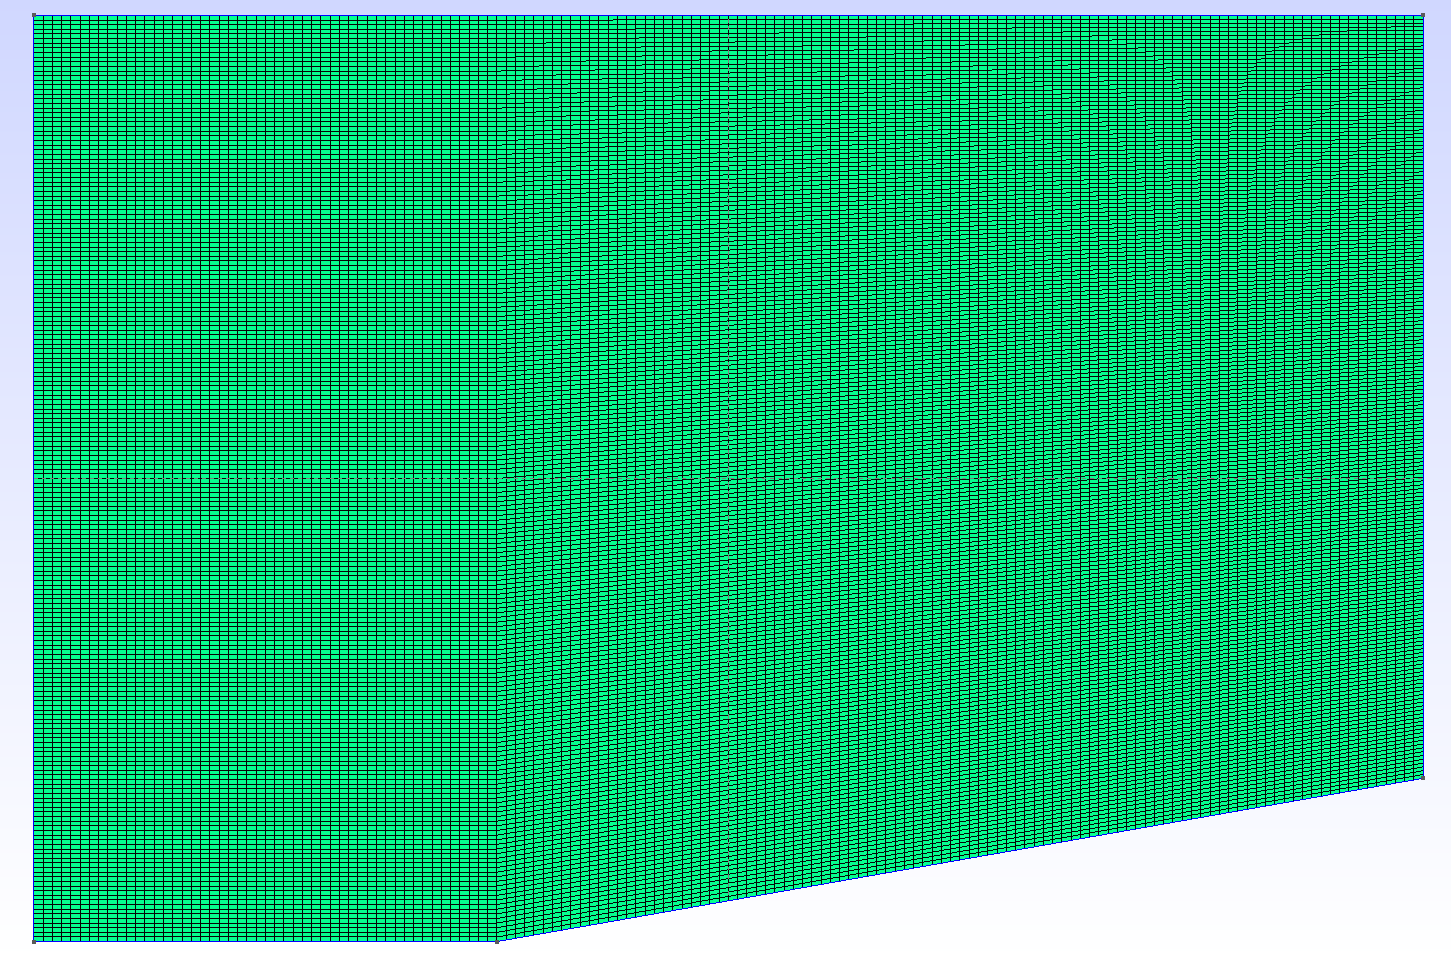
\includegraphics[width=0.8\textwidth]{text/inviscid_wedge_fine_mesh.png}\\
\caption[Inviscid Mesh]{Mesh: 30,000 Cells | Generated in Gmsh}
\label{fig1.1: Inviscid Mesh}
\end{figure}
\\
\begin{figure}[H]
\centering
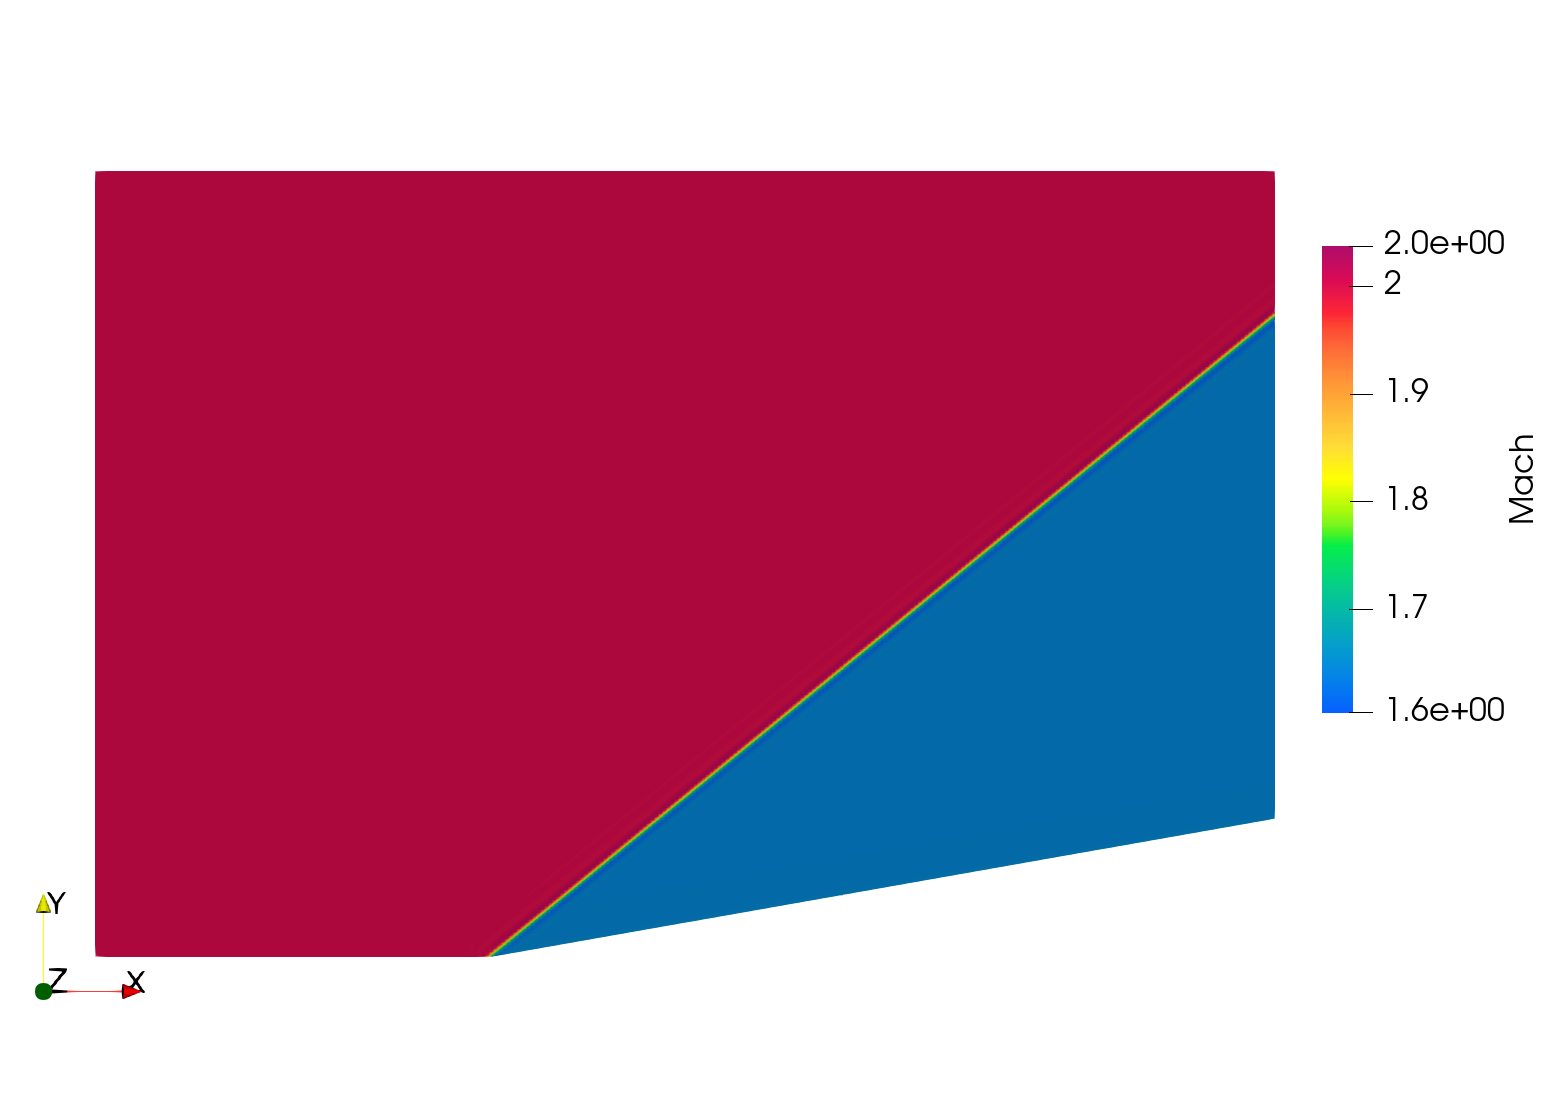
\includegraphics[width=0.8\textwidth]{text/Mach_HLLC_Inviscid_Wedge.png}\\
\caption[Inviscid Mach Contour]{Mach Contour}
\label{fig: Inviscid Mach Contour}
\end{figure}

\begin{figure}[H]
\centering
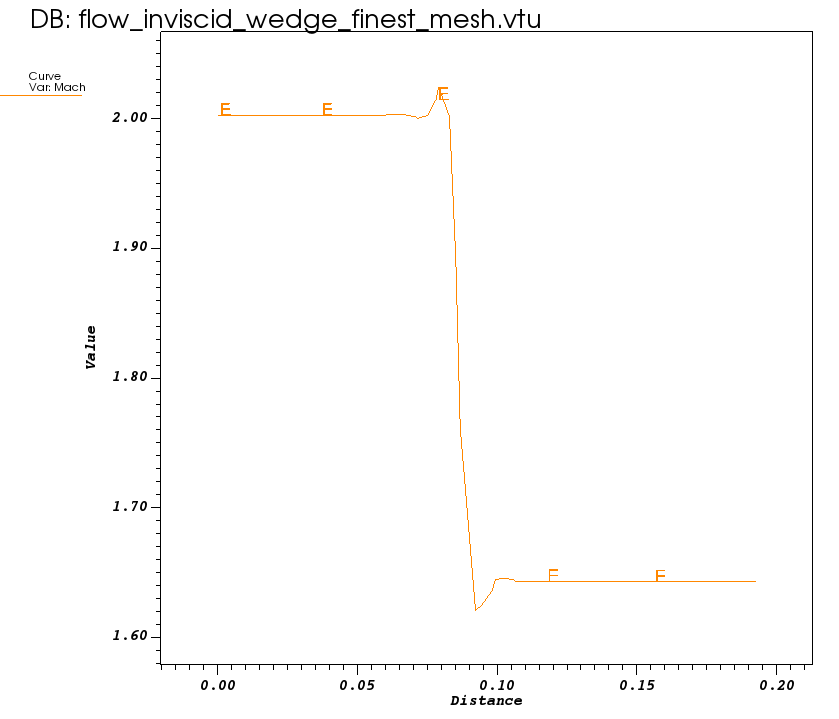
\includegraphics[width=0.6\textwidth]{text/Mach_Per_Shock_Inviscid_Wedge.png}\\
\caption[HLLC - Mach vs. X]{HLLC - Mach vs. X}
\label{fig: Mach vs. X}
\end{figure}

\begin{figure}[H]
\centering
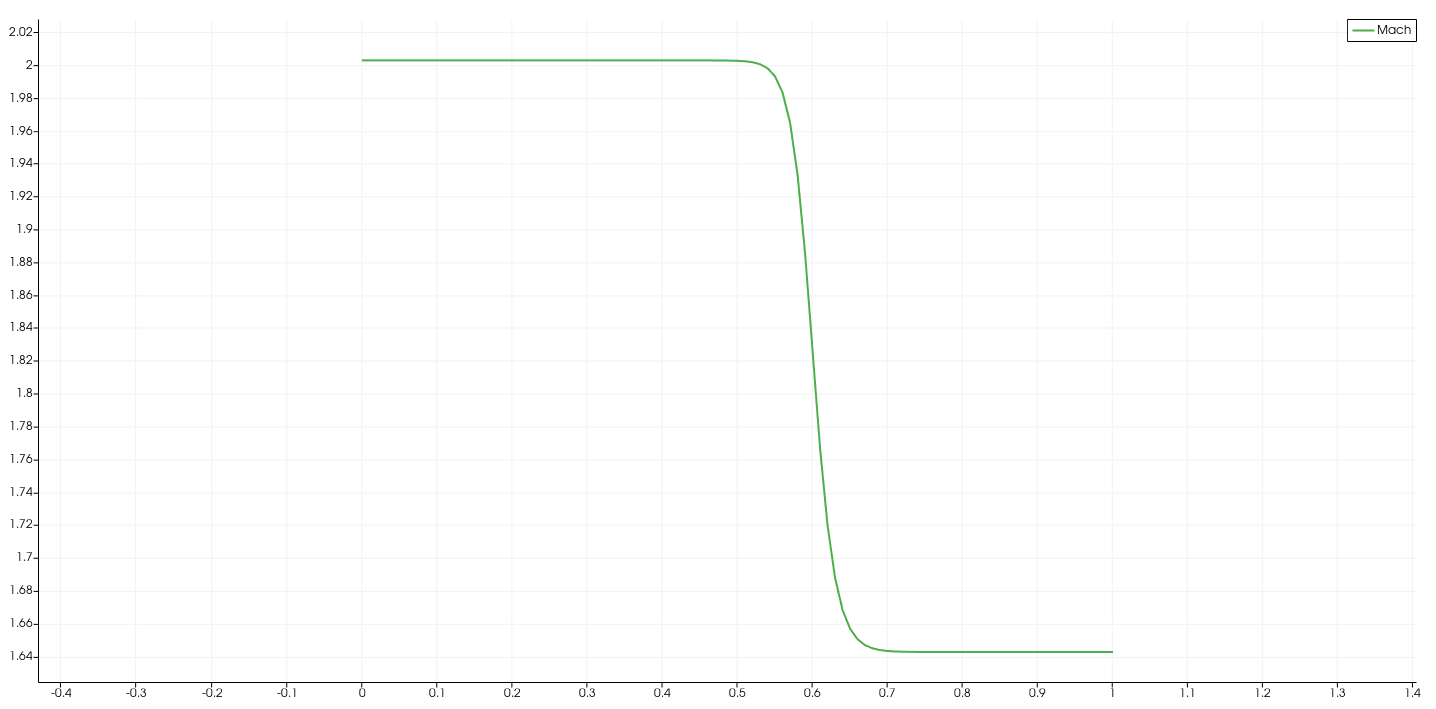
\includegraphics[width=0.8\textwidth]{text/Lax_M_vs_X_Inviscid_Wedge.png}\\
\caption[Lax-Friedrich - Mach vs. X]{Lax-Friedrich - Mach vs. X}
\label{fig: Lax-Friedrich - Mach vs. X}
\end{figure}
\\
Post-Processing: The theoretical value of shock angle is $39.314^0$, but the value from the simulation is $40.019^0$. This was found using the density gradient, where the maximum value of the gradient was calculated at the shock, since the maximum gradient has to be perpendicular to the shock, $90^0$ was added to the gradient angle to find the shock angle. The shock angle was averaged over four such values calculated from five different horizontal lines passing through the shock with a spacing of 0.005 units along the y-axis. The error in shock angle is 1.80\%. \\
\begin{center}
$ \triangledown \rho = \frac{d\rho}{dx} \hat{i} + \frac{d\rho}{dy} \hat{j}  $\\
$ |\triangledown \rho| = \sqrt{(\frac{d\rho}{dx})^2  + (\frac{d\rho}{dy})^2 } $ \\
$ \theta_{shock} = \frac{\pi}{2} + \arctan{(\frac{d\rho/dy}{d\rho/dx})}$ at $|\triangledown \rho|_{max} $
\end{center}
\newpage
The data from the numerical schemes were extracted and plotted for comparison
\begin{figure}[H]
    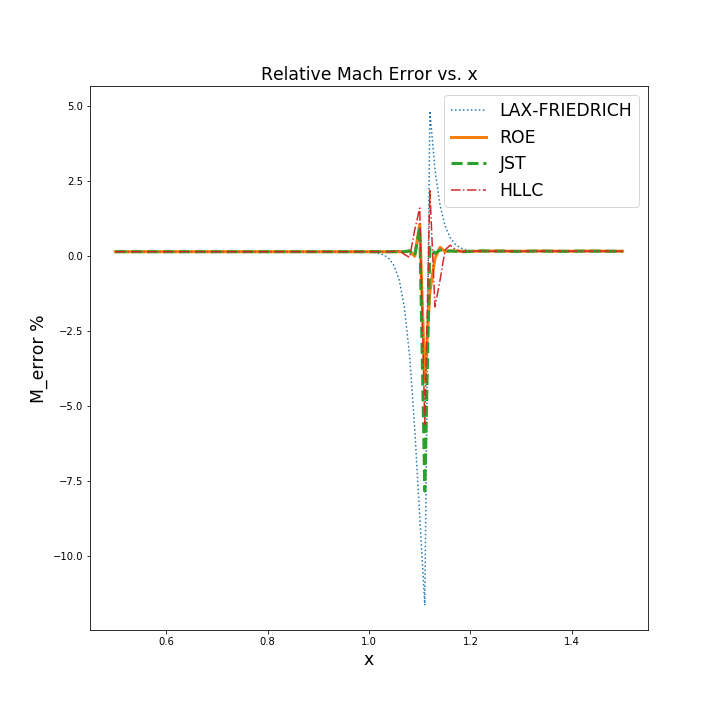
\includegraphics[width=0.5\textwidth]{text/M_error_comparison.png}
    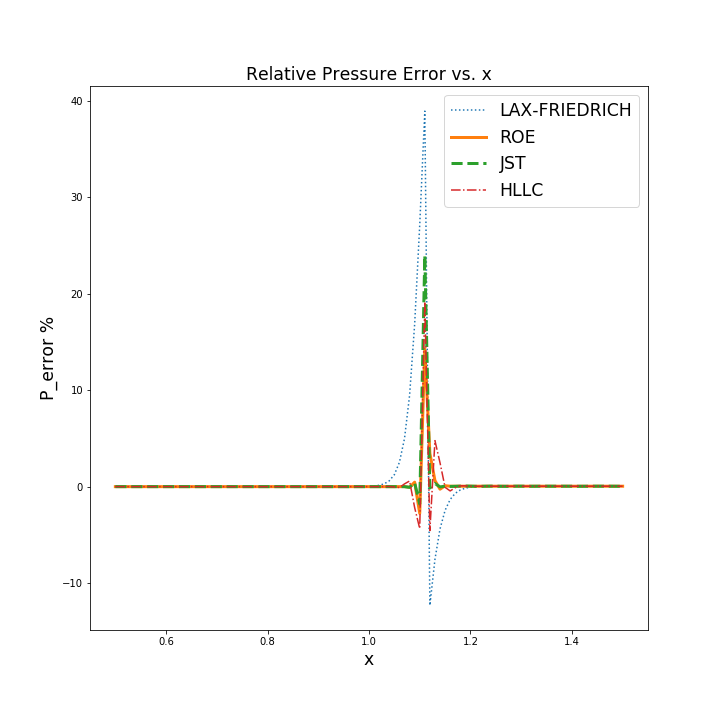
\includegraphics[width=0.5\textwidth]{text/P_error_comparison.png}
    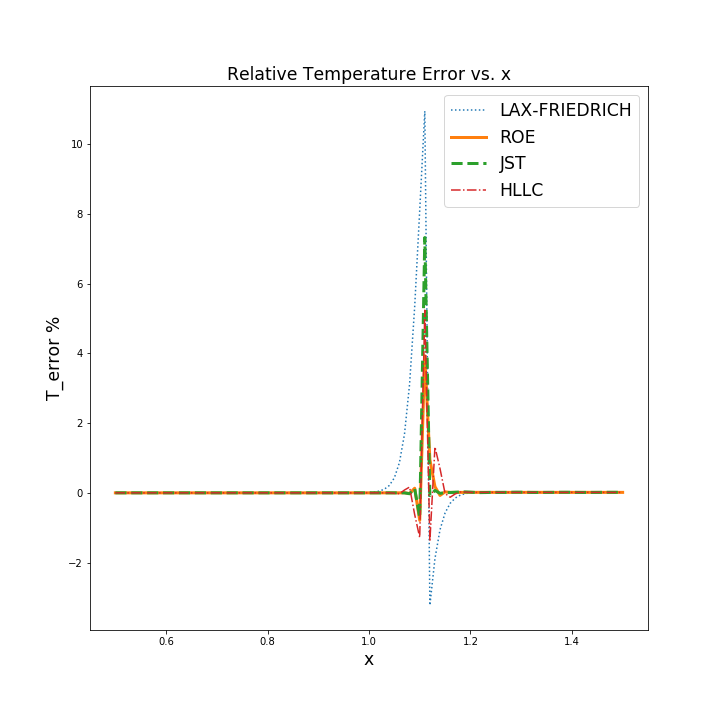
\includegraphics[width=0.5\textwidth]{text/T_error_comparison.png}
    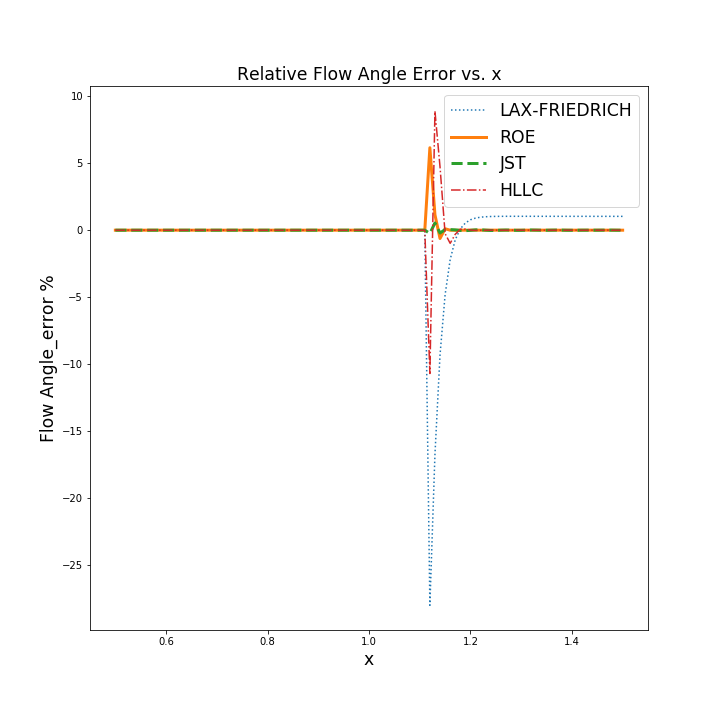
\includegraphics[width=0.5\textwidth]{text/FA_error_comparison.png}
    \caption[Errors associated with the Numerical Scheme]{Errors associated with the Numerical Scheme}
    \label{fig:Errors associated with the Numerical Scheme}
\end{figure}
From the plots shown above the ROE scheme seems to have the least error, followed by the HLLC scheme, but it is computationally expensive, so the HLLC scheme was chosen for its faster convergence and accurate results\\
\begin{table}[h]
    \centering
    \begin{tabular}{|l|l|l|l|l|l|}
    \hline
    Convective NM & M_2 & P_2 & T_2 & Time(sec)\\
    \hline
    JST & 1.643XX & 1707XX & 351.0XX & 644.16\\
    \hline
    LAX\_FRIEDRICH & 1.642XX & 17075X & 351.XXX & 197.6\\
    \hline
    HLLC & 1.6431X & 17073X & 351.09X & 106.75\\
    \hline
    ROE & 1.6431X & 17073X & 351.09X & 553.2\\
    \hline
\end{tabular}
    \caption{Comparison between Convective NM}
    \label{tab:Comparisonbetween Convective NM }
\end{table}
\newpage
\begin{figure}
    \centering
    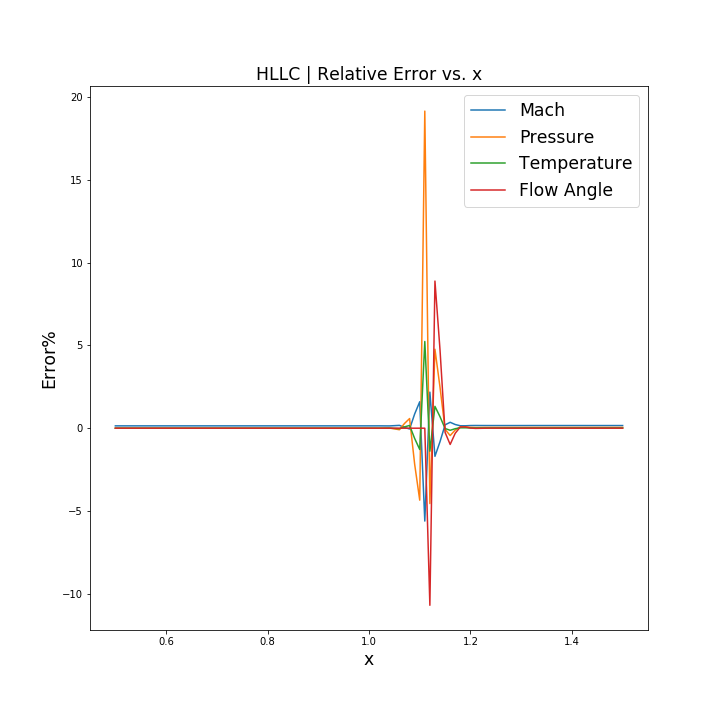
\includegraphics[width=0.75\textwidth]{text/error_HLLC.png}   
    \caption[HLLC - Relative Error]{Relative Error in flow variables}
    \label{fig:HLLC - Relative Error}
\end{figure}

\subsection{Time vs. CFL}
In this section, for a constant number of cells, the optimum CFL number is found by plotting Time vs. CFL number, which has the minimum computational cost. And then the number of mesh cells is quadrupled to test if the same trend continues.\\
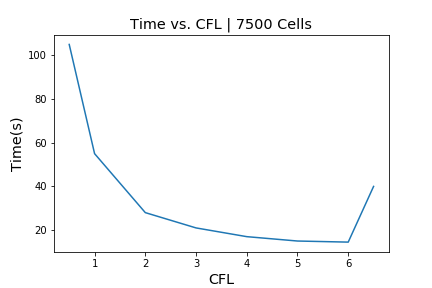
\includegraphics[width=0.5\textwidth]{text/time_vs_CFL_7500_Cells.png}
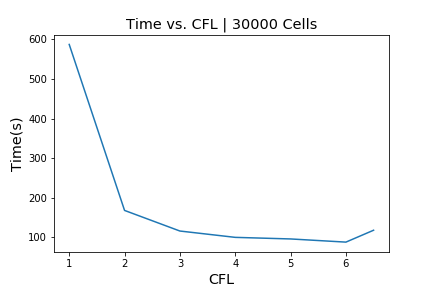
\includegraphics[width=0.5\textwidth]{text/time_vs_CFL_30000_Cells.png}\\
For CFL values lesser than 1, the convergence is so slow that even after 10000 iterations the residual were far from the convergence criteria. For CFL values greater than 7, the residual initially oscillates around and then later diverges.\\
\newpage